\section{Extension to Multi-Chaser Systems}
\label{sec:multi-agent}
Although several uncontrollable objects in orbit are relatively small, some of the most concerning ones (with respect to the risk they pose to vital controllable systems) are large rocket bodies \cite{mcknight2021identifying}.
A single chaser that may be as large as a conventional satellite may not be capable of providing sufficient thrust or leverage to detumble such an object.
As a result, we propose the use of multiple chasers to simultaneously act on the target for tumble minimization and deorbiting.
In the process of rendezvous and docking, such a multi-agent system will require additional constraints to prevent collisions between themselves and the allocation of similar docking positions on the target.\\
% Furthermore, during rendezvous, it may be optimal for the chasers to view the target from different angles to maximize information regarding the shape and inertial parameters of the target to decide docking points for the chasers.
% We address the addition of inter-chaser constraints and basic observation techniques in this section.
% \subsection{Modifications to the Rendezvous and Docking Problem}
The separate implementation of the rendezvous and docking problem proposed in Sections \ref{sec:chaser_ampc} and \ref{sec:constraints} for each chaser in a multi-agent context introduces the risk of collisions between chasers along with the already-addressed issue of collisions between the chaser and the target as well as the possibility of multiple chasers picking the same docking point.
For the multi-agent problem, the split-up problem of distributed optimization followed by distributed task/goal allocation followed by individual trajectory planning may be different in solution and hence in optimality from the combined problem of distributed optimal control.
The former fails to consider the position of non-ego agents for each individual trajectory planning problem, hence posing the risk of collision.
As a result, we suggest the use of the combined problem of distributed optimal control where the same problem is solved by each chaser based on the initial state of all chasers and a common final state manifold.
Moreover, the problem requires focusing on minimizing the total cost of the operation instead of the individual costs of each chaser.
On the other hand, this brings up the possibility of resource depletion for individual chasers due to which the total control input over time needs to be constrained.
As a result, the multi-agent problem for rendezvous can be written as follows:
\begin{align}
    \min_{\boldsymbol{r}, \boldsymbol{u}}\quad &J(\boldsymbol{r}(\theta),\boldsymbol{u}(\theta))\\
    & =\sum_{i=1}^{N_C}\Big(h(\boldsymbol{r}_i(\theta_f))\notag\\
    & \quad\ +\int_{\theta_0}^{\theta_f}\left(\boldsymbol{r}_i^T(\theta)Q_i\boldsymbol{r}_i(\theta)+\boldsymbol{u}_i^T(\theta)R_i\boldsymbol{u}_i(\theta)\right)d\theta\Big)\notag
\end{align}
\begin{subequations}
\begin{align}
    \textrm{s.t. } & \boldsymbol{r}_i'(\theta)=A(\theta)\boldsymbol{r}_i(\theta)+B(\theta)\boldsymbol{u}_i(\theta)+\boldsymbol{d}(\theta),\\
    & \boldsymbol{r}_i(\theta_0)={\boldsymbol{r}}_{i,0},\quad\quad\boldsymbol{u}_i\in{\mathbb{U}}_i,\\
    & \boldsymbol{r}(\theta)\in{\mathcal{C}}_{i,T}\qquad\quad\ \boldsymbol{r}(\theta)\in{\mathcal{C}}_{i,j}\label{eqn:multi-agent-rendezvous}
\end{align}
\end{subequations}
where $i,j\in[1,2,\ldots,N_C]$ and $j>i$.
Here, while the chaser-target collision constraints, ${\mathcal{C}}_{i,T}$, can be expanded as explained in Section \ref{sec:time-varying-collision-constraints}, the inter-chaser collision constraints can be written as follows:
\begin{align}
    {\mathcal{C}}_{i,j}&=\{\boldsymbol{r}_i(\theta):||\boldsymbol{r}^P_{i}-\boldsymbol{r}^P_{j}||-\epsilon_{i,j}\}
\end{align}
where $\epsilon_{i,j}$ is predetermined based on the geometry of chasers $i$ and $j$. A similar multi-agent problem can be written for the docking problem by replacing the chaser-target collision constraint accordingly.

% \subsection{Observation Shape and Size} \label{ssec:observation-shape}
% Although we propose the optimal positioning of chasers for the observation of and approach toward the target, we employ existing techniques such as that proposed in \cite{setterfield2018inertial} for the estimation of inertial parameters of the target.

% \subsection{Individual Goal State Determination} \label{ssec:goal-state-determination}
% The goal state (position and velocity) of each chaser is determined to lie on an observation sphere of optimal radius as discussed in Section \ref{ssec:observation-shape}

\iffalse{
\subsection{Observation Shape and Size}
\label{sec:obs_sphere}
Before the final step of docking with the target, in order to obtain information regarding the mass, moment of inertia, possible locations for docking, and other quantities pertaining to the target vital for the operation, the rendezvous problem may involve intermediate goal points on progressively shrinking concentric surfaces as depicted in Fig. \ref{fig:obs_spheres}.
\begin{figure}[hbt!]
    \centering
    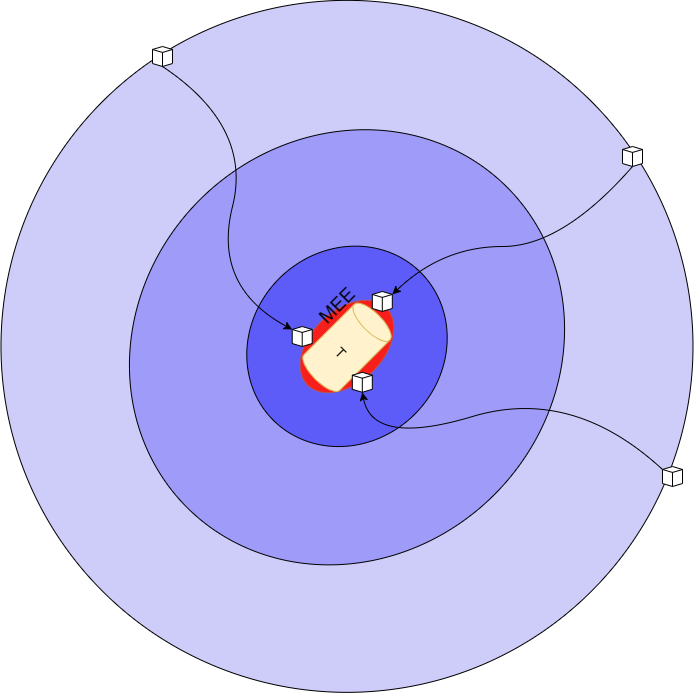
\includegraphics[width=.75\linewidth]{assets/obs-spheres.png}
    \caption{\textbf{Observation and Approach of Chasers onto the Target.} The chasers collect and share information regarding the target as they approach it at each observation surface.}
    \label{fig:obs_spheres}
\end{figure}
In order to calculate optimal positions for chasers to observe the target, we propose a nonlinear optimization problem that aims to maximize the observability of the target.
We draw motivation from multi-satellite implementations for remote sensing and similar works \cite{chen2020a,gu2023large} to define the observability of the target as a heuristic that is proportional to the fraction of area of the target that is observed.
It is easy to realize that the fraction of observed area is proportional to the spread between the chasers at any fixed distance from the target.
% Moreover, given a fixed number of concentric observation surfaces, it may be preferable to distribute the surfaces as far from each other as possible to support easier transit from one surface to the next.
As a result, we define observability as follows while encouraging the reader to explore the possibility of more optimal measurements of observation:
\begin{align}
    {\mathcal{O}}&=Q_{\text{local}}{\mathcal{O}}_{\text{local}}+Q_{\text{cross}}{\mathcal{O}}_{\text{cross}}\\
    {\mathcal{O}}_{\text{local}}&=\sum_{l=1}^{N_L}\sum_{i=1}^{N_C}\sum_{j=i}^{N_C}\left(||\boldsymbol{r}_{i,l}^P-\boldsymbol{r}_{j,l}^P||\right)\\
    {\mathcal{O}}_{\text{cross}}&=\sum_{l=2}^{N_L}\sum_{i=1}^{N_C}\left(-||\boldsymbol{r}_{i,l}^P-\boldsymbol{r}_{i,l-1}^P||\right)
\end{align}
where $\boldsymbol{r}_{i,l}^P$ is the position (in all three axes) of agent $i$ at the $l$th observation surface.
% \begin{equation}
%     \mathcal{O}(\mathcal{S}, \{p_i(t)\forall i\in\mathbb{N}\}(t) \begin{cases} < 1 &\text{for a net loss of information}\\
%                                                                                = 1 &\text{for no net gain or loss of information}\\
%                                                                                > 1 &\text{for a net gain of information}
%                                                                  \end{cases}
% \end{equation}

Now, with the ellipsoid ${\mathcal{E}}_T$ of parameters $a_T, b_T, c_T$ as the final state constraints and a starting ellipsoid ${\mathcal{E}}_0$ of parameters $a_0, b_0, c_0$ such that all the chasers start from points that lie on $\mathcal{E}_0$, we solve the following minimization problem to obtain the optimal observation ellipsoids:
\begin{equation}
\begin{aligned}
    \min_{a_l, b_l, c_l}\quad &J_E=\sum_{l=1}^{N_L-1}{\mathcal{O}}({\mathcal{E}}_l, \{p_{i,l} \forall\ i\in{\mathbb{N}}_C\})\\
    \textrm{s.t. } & a_{l}\leq a_{l-1},\ \ b_{l}\leq b_{l-1},\ \  c_{l}\leq c_{l-1},\ \ \forall\ l\in{\mathbb{N}}_L\\
    & \frac{x_{i,l}^2}{a_l^2}+\frac{y_{i,l}^2}{b_l^2}+\frac{z_{i,l}^2}{c_l^2}=1\ \ \forall\ i\in{\mathbb{N}}_C, l\in{\mathbb{N}}_L
    \label{eqn:mee}
\end{aligned}
\end{equation}
Although we propose the optimal positioning of chasers for the observation of the target and their approach to the target, we employ existing techniques such as those proposed in \cite{setterfield2018inertial} for the estimation of the inertial parameters of the target.
}
% \begin{figure*}
% \centering
% \includegraphics[width=4in]{Placeholder.eps}
% \caption{\bf{Here is an example of a figure that spans both columns.}}
% \label{FlowChart}
% \end{figure*}

% \begin{table}
% \renewcommand{\arraystretch}{1.3}
% \caption{\bf Summary of Due Dates}
% \label{DueDates}
% \centering
% \begin{tabular}{|c|c|}
% \hline
% \bfseries Event & \bfseries Due Date \\
% \hline\hline
% Abstracts Due               & July 1, 2023 \\
% Draft Paper {\bf Deadline} & October 6, 2023 \\
% Revised papers Due          & January 12, 2024\\
% IEEE Copyright Form Due     & January 12, 2024\\
% \hline
% \end{tabular}
% \end{table}